% assignment_2.tex
% CS 8735 - Unsupervised Learning (Fall 2015)
%     University of Missouri-Columbia
%             Chanmann Lim
%            October 2015

\documentclass[a4paper]{article}

\usepackage[margin=1 in]{geometry}
\usepackage{listings}
\usepackage{amsmath}
\usepackage{graphicx}
\usepackage{float}
\usepackage{multirow}

\everymath{\displaystyle}
\DeclareMathOperator*{\argmax}{\arg\!\max}
\DeclareMathOperator*{\argmin}{\arg\!\min}

\begin{document}
\setcounter{page}{6}

\noindent The Matlab code for all experiments is in the \textbf{Appendix} section.

\paragraph{6.d.} The goal of this problem is to investigate the influences of the ordering of the dataset in sequential clustering algorithm namely \emph{Basic Sequential Algorithmic Scheme (BSAS)} and \emph{Modified Basic Sequential Algorithmic Scheme (MBSAS)}. According to the literature, the main difference between BSAS and MBSAS is that the latter separates the clustering procedure into two parts. Firstly, the class determination phase is served as cluster discovery stage to find out the possible number of clusters with the constraints $\Theta$ : the distance threshold to subsume a data point to a cluster and $q$ : the numbers of maximum allowed clusters. Secondly, the pattern classification stage where each point is being assigned to one of the already created clusters. \\

	\underline{Plot of the vectors:}
	
	\begin{figure}[H]
	  \centering
	    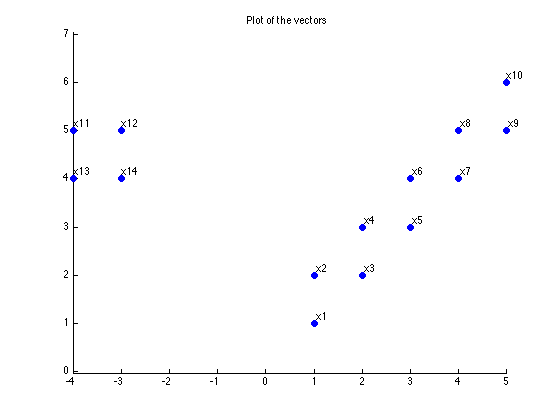
\includegraphics[scale=.57]{images/vectors.png}
	  \caption{Plot of vectors}
	\end{figure}

	For case \textbf{a.} where the ordering of the dataset is $\mathbf{x}_1, \mathbf{x}_2,\cdots, \mathbf{x}_{14}$ we got:
	
	$$BSAS = \{
		\{ \mathbf{x}_1,  \mathbf{x}_2,  \mathbf{x}_3 \},     
		\{ \mathbf{x}_4,  \mathbf{x}_5,  \mathbf{x}_6 \},     
		\{ \mathbf{x}_7,  \mathbf{x}_8,  \mathbf{x}_9 \},     
		\{ \mathbf{x}_{10} \},     
		\{ \mathbf{x}_{11},  \mathbf{x}_{12},  \mathbf{x}_{13},  \mathbf{x}_{14} \}
	\}$$
	$$MBSAS = \{
		\{ \mathbf{x}_1,  \mathbf{x}_2 \},     
		\{ \mathbf{x}_4,  \mathbf{x}_3,  \mathbf{x}_5 \},     
		\{ \mathbf{x}_7,  \mathbf{x}_6,  \mathbf{x}_8 \},     
		\{ \mathbf{x}_{10},  \mathbf{x}_9 \},     
		\{ \mathbf{x}_{11},  \mathbf{x}_{12},  \mathbf{x}_{13},  \mathbf{x}_{14} \}
	\}$$
	
	\noindent The reason of the difference being MBSAS is trying to balance out the cluster assignment decision until all possible clusters are identified. This solves the problem with BSAS which decided a vector $\mathbf{x}$ to belong to an already created cluster or a new cluster prior to the final cluster formation. \\
	
	For case \textbf{b.} where the ordering of the dataset is $\mathbf{x}_{1},   \mathbf{x}_{10},    \mathbf{x}_{2},    \mathbf{x}_{3},    \mathbf{x}_{4},   \mathbf{x}_{11},   \mathbf{x}_{12},    \mathbf{x}_{5},    \mathbf{x}_{6},    \mathbf{x}_{7},   \mathbf{x}_{13},     \mathbf{x}_{8},   \mathbf{x}_{14},    \mathbf{x}_{9}$ and the clusters obtained:
	
	$$BSAS = \{ \{ \mathbf{x}_{1}, \mathbf{x}_{2}, \mathbf{x}_{3} \},    
		\{ \mathbf{x}_{10}, \mathbf{x}_{9} \},    
		\{ \mathbf{x}_{4}, \mathbf{x}_{5}, \mathbf{x}_{6} \},    
		\{ \mathbf{x}_{11}, \mathbf{x}_{12}, \mathbf{x}_{13}, \mathbf{x}_{14} \},    
		\{ \mathbf{x}_{7}, \mathbf{x}_{8} \} \}$$
	$$MBSAS = \{ \{ \mathbf{x}_{1},  \mathbf{x}_{2} \},    
		\{ \mathbf{x}_{10},  \mathbf{x}_{9} \},    
		\{ \mathbf{x}_{4},  \mathbf{x}_{3},  \mathbf{x}_{5} \},    
		\{ \mathbf{x}_{11},  \mathbf{x}_{12},  \mathbf{x}_{13},  \mathbf{x}_{14} \},    
		\{ \mathbf{x}_{7},  \mathbf{x}_{6},  \mathbf{x}_{8} \} \}$$
		
	For case \textbf{c.} where the ordering of the dataset is $\mathbf{x}_{1},    \mathbf{x}_{10},     \mathbf{x}_{5},     \mathbf{x}_{2},     \mathbf{x}_{3},    \mathbf{x}_{11},    \mathbf{x}_{12},     \mathbf{x}_{4},     \mathbf{x}_{6},     \mathbf{x}_{7},    \mathbf{x}_{13}    \mathbf{x}_{14},     \mathbf{x}_{8},     \mathbf{x}_{9}$ and the clusters obtained:
	
	$$BSAS = \{ \{ \mathbf{x}_{1},  \mathbf{x}_{2},  \mathbf{x}_{3} \},     
		\{ \mathbf{x}_{10},  \mathbf{x}_{9} \},     
		\{ \mathbf{x}_{5},  \mathbf{x}_{4},  \mathbf{x}_{6} \},     
		\{ \mathbf{x}_{11},  \mathbf{x}_{12},  \mathbf{x}_{13},  \mathbf{x}_{14} \},     
		\{ \mathbf{x}_{7},  \mathbf{x}_{8} \} \}$$
	$$MBSAS = \{ \{ \mathbf{x}_{1},  \mathbf{x}_{2},  \mathbf{x}_{3} \},     
		\{ \mathbf{x}_{10},  \mathbf{x}_{8},  \mathbf{x}_{9} \},     
		\{ \mathbf{x}_{5},  \mathbf{x}_{4},  \mathbf{x}_{6},  \mathbf{x}_{7} \},     
		\{ \mathbf{x}_{11},  \mathbf{x}_{12},  \mathbf{x}_{13},  \mathbf{x}_{14} \} \}$$

	\noindent In the last case MBSAS looked through the data and suggested only four clusters conversely BSAS purely depended on the ordering the data set and formed a total of five clusters. \\
	
\paragraph{6.e.} From the plot of the vectors we can claim that there are 2 basic clusters from visual clustering of the data. \\

	$$ C = \{ \{\mathbf{x}_{1}, \mathbf{x}_{2}, \mathbf{x}_{3}, \mathbf{x}_{4}, \mathbf{x}_{5}, \mathbf{x}_{6}, \mathbf{x}_{7}, \mathbf{x}_{8}, \mathbf{x}_{9}, \mathbf{x}_{10} \}, 
	\{\mathbf{x}_{11}, \mathbf{x}_{12}, \mathbf{x}_{13}, \mathbf{x}_{14}\} \} $$
	
\paragraph{7.} In this task we are performing \textbf{k-mean} clustering with $k = 4$ on the GMD dataset from previous assignment. We started by initializing the centroids of all clusters randomly between -1 and 10 (empirically selected range and it doesn't carry out any knowledge-based implication) then run k-mean algorithm which consists of cluster assignment step in which a sample is assigned to closest cluster $C_{k_n^{\ast}}$.

	\begin{equation}
		k_n^{\ast} = \argmin_k \|x_n - \mu_k\|^2
	\end{equation}
	
	After all samples are assigned to clusters then update the cluster centroids by replacing it with the mean of the samples belong to each cluster $k$.
	
	\begin{equation}
		\hat{\mu_k} = \frac{1}{|C_k|} \sum_{x_n \in C_k} x_n \qquad	; k=1,2,3,4
	\end{equation}
	
	Finally, we compute the total distortion scores and check if it is unchanged(converged) then stop k-mean otherwise repeat the cluster assignment and centroid update until convergence. \\
	
\paragraph{7.1} The randomly initialization gave us: \\

	\begin{align}
		U^{(0)} &= \begin{bmatrix}
				\mu_{1,1}  &  \mu_{2,1}  &  \mu_{3,1}  &  \mu_{4,1} \\ 
			    \mu_{1,2}  &  \mu_{2,2}  &  \mu_{3,2}  &  \mu_{4,2}
			\end{bmatrix} \\
			&= \begin{bmatrix}
				5.5742  &  8.8840  &  7.9968  &  7.1754 \\ 
			    4.2734  &  9.2818  &  6.7980  &  8.8968
			\end{bmatrix}
	\end{align}
	
	And the final cluster centroids is: 
	
	\begin{align}
		U &= \begin{bmatrix}
				1.3781  &  9.2459  & 13.1269  &  4.8156 \\ 
			    1.7408  &  6.6790  &  2.8714  &  6.5621
			\end{bmatrix}
	\end{align}

\paragraph{7.2} The plot of samples with clusters: \\

	\begin{figure}[H]
	  \centering
	    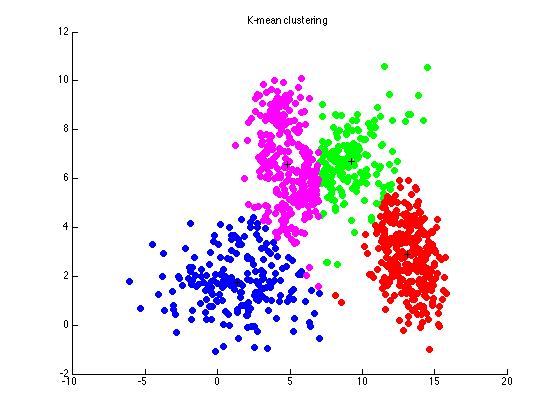
\includegraphics[scale=.57]{images/k_mean.png}
	  \caption{Plot of samples with clusters}
	\end{figure}

\paragraph{7.3} The total distortion are [10154,    6105,    4869,    4675,    4652,    4648,    4647,    4647]. \\

	\begin{figure}[H]
	  \centering
	    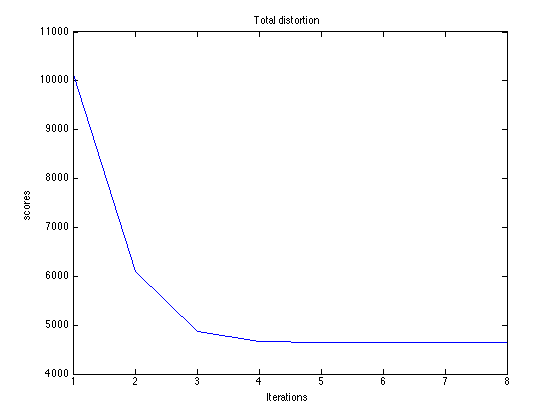
\includegraphics[scale=.57]{images/distortion.png}
	  \caption{Total distortion}
	\end{figure}
	
\paragraph{Epilogue: } K-mean is simply a special case of EM algorithm with the assumption that the prior probability is uniform $\pi_k = \frac{1}{k}$ and all clusters have the same covariance matrix $\Sigma_k = \sigma^2 \cdot \mathbf{I} \quad; k=1,2,...,K$. Unlike EM it imposes hard clustering which make it converge faster and consume less computation than EM, yet k-mean and EM relay very strongly on good initialization and if k-mean somehow landed on a bad initialization it will also diverge faster than EM algorithm.

\newpage
\subsection*{Appendix:}
	\lstinputlisting[language=Matlab, title=\lstname, basicstyle=\footnotesize]{assignment_2.m}
	\lstinputlisting[language=Matlab, title=\lstname, basicstyle=\footnotesize]{problem_6.m}
	\lstinputlisting[language=Matlab, title=\lstname, basicstyle=\footnotesize]{problem_7.m}	
	\lstinputlisting[language=Matlab, title=\lstname, basicstyle=\footnotesize]{bsas.m}
	\lstinputlisting[language=Matlab, title=\lstname, basicstyle=\footnotesize]{mbsas.m}
	\lstinputlisting[language=Matlab, title=\lstname, basicstyle=\footnotesize]{min_distance.m}
	\lstinputlisting[language=Matlab, title=\lstname, basicstyle=\footnotesize]{print_cluster.m}
	\lstinputlisting[language=Matlab, title=\lstname, basicstyle=\footnotesize]{k_mean.m}	
\end{document}